%% abtex2-modelo-trabalho-academico.tex, v-1.9.2 laurocesar
%% Copyright 2012-2014 by abnTeX2 group at http://abntex2.googlecode.com/ 
%%
%% This work may be distributed and/or modified under the
%% conditions of the LaTeX Project Public License, either version 1.3
%% of this license or (at your option) any later version.
%% The latest version of this license is in
%%   http://www.latex-project.org/lppl.txt
%% and version 1.3 or later is part of all distributions of LaTeX
%% version 2005/12/01 or later.
%%
%% This work has the LPPL maintenance status `maintained'.
%% 
%% The Current Maintainer of this work is the abnTeX2 team, led
%% by Lauro César Araujo. Further information are available on 
%% http://abntex2.googlecode.com/
%%
%% This work consists of the files abntex2-modelo-trabalho-academico.tex,
%% abntex2-modelo-include-comandos and abntex2-modelo-references.bib
%%

% ------------------------------------------------------------------------

\documentclass[
	% -- opções da classe memoir --
	12pt,				% tamanho da fonte
	% openright,			% capítulos começam em pág ímpar (insere página vazia caso preciso)
	oneside,			% para impressão apenas no anverso (apenas frente). Oposto a twoside
	a4paper,			% tamanho do papel. 
	% -- opções da classe abntex2 --
	%chapter=TITLE,		% títulos de capítulos convertidos em letras maiúsculas
	%section=TITLE,		% títulos de seções convertidos em letras maiúsculas
	%subsection=TITLE,	% títulos de subseções convertidos em letras maiúsculas
	%subsubsection=TITLE,% títulos de subsubseções convertidos em letras maiúsculas
	% -- opções do pacote babel --
	english,			% idioma adicional para hifenização
	%french,				% idioma adicional para hifenização
	%spanish,			% idioma adicional para hifenização
	brazil				% o último idioma é o principal do documento
	]{abntex2ppgsi}

% ---
% Pacotes básicos 
% ---
% \usepackage{lmodern}			% Usa a fonte Latin Modern			
% \usepackage[T1]{fontenc}		% Selecao de codigos de fonte.
\usepackage[utf8]{inputenc}		% Codificacao do documento (conversão automática dos acentos)
\usepackage{indentfirst}		% Indenta o primeiro parágrafo de cada seção.
\usepackage{color}				% Controle das cores
\usepackage{graphicx}			% Inclusão de gráficos
\usepackage{microtype} 			% para melhorias de justificação
\usepackage{pdfpages}     %para incluir pdf
\usepackage{algorithm}			%para ilustrações do tipo algoritmo
\usepackage{mdwlist}			%para itens com espaço padrão da abnt
\usepackage[noend]{algpseudocode}			%para ilustrações do tipo algoritmo
		
% ---
% Pacotes adicionais, usados apenas no âmbito do Modelo Canônico do abnteX2
% ---
%\usepackage{lipsum}				% para geração de dummy text
% ---

% ---
% Pacotes de citações
% ---
\usepackage[brazilian,hyperpageref]{backref}	 % Paginas com as citações na bibl
\usepackage[alf]{abntex2cite}	% Citações padrão ABNT

% --- 
% CONFIGURAÇÕES DE PACOTES
% --- 

% ---
% Configurações do pacote backref
% Usado sem a opção hyperpageref de backref
\renewcommand{\backrefpagesname}{Citado na(s) página(s):~}
% Texto padrão antes do número das páginas
\renewcommand{\backref}{}
% Define os textos da citação
\renewcommand*{\backrefalt}[4]{
	\ifcase #1 %
		Nenhuma citação no texto.%
	\or
		Citado na página #2.%
	\else
		Citado #1 vezes nas páginas #2.%
	\fi}%
% ---

% ---
% Informações de dados para CAPA e FOLHA DE ROSTO
% ---

%-------------------------------------------------------------------------
\instituicao{
	UNIVERSIDADE DE SÃO PAULO
	\par
	ESCOLA DE ARTES, CIÊNCIAS E HUMANIDADES
	\par
	PROJETO SUPERVISIONADO DE GRADUAÇÃO II - ACH 2018}

%-------------------------------------------------------------------------

%-------------------------------------------------------------------------
% Informações sobre o ``título'':
%
% Em maiúscula apenas a primeira letra da sentença (do título), exceto 
% nomes próprios, geográficos, institucionais ou Programas ou Projetos ou 
% siglas, os quais podem ter letras em maiúscula também.
%
% O subtítulo do trabalho é opcional.
% Sem ponto final.
%-------------------------------------------------------------------------
\titulo{Efeitos do 'Filtro Bolha' e do Viés de Confirmação na esfera pública atual}

%-------------------------------------------------------------------------
% Informações sobre o ``autor'':
%
% Todas as letras em maiúsculas.
% Nome completo.
% Sem ponto final.
%-------------------------------------------------------------------------
\autor{\uppercase{BRUNO IMPOSSINATO MUROZAKI}}

%-------------------------------------------------------------------------
% Informações sobre o ``local'':
%
% Não incluir o ``estado''.
% Sem ponto final.
%-------------------------------------------------------------------------
\local{São Paulo}

%-------------------------------------------------------------------------
% Informações sobre a ``data'':
%
% Colocar o ano do depósito (ou seja, o ano da entrega). 
%
% Não incluir o dia, nem o mês.
% Sem ponto final.
%-------------------------------------------------------------------------
\data{2018}

%-------------------------------------------------------------------------
% Informações sobre o ``Orientador'':
%
% Se for uma professora, trocar por ``Profa. Dra.''
% Nome completo.
% Sem ponto final.
%-------------------------------------------------------------------------
\orientador{Prof. Doutor Márcio Moretto}
%-------------------------------------------------------------------------
\tipotrabalho{Disciplina Projeto Supervisionado de Graduação II - ACH 2018}

\preambulo{
%-------------------------------------------------------------------------
% Versão original \newline \newline \newline
%-------------------------------------------------------------------------
 Monografia apresentada à Escola de Artes, Ciências e Humanidades da Universidade de São Paulo como requisito para a disciplina Projeto Supervisionado de Graduação II - ACH 2018, para a obtenção do título de Bacharel em Sistemas de Informação.
}
%-------------------------------------------------------------------------
% Configurações de aparência do PDF final

% alterando o aspecto da cor azul
\definecolor{blue}{RGB}{41,5,195}

% informações do PDF
\makeatletter
\hypersetup{
     	%pagebackref=true,
		pdftitle={\@title}, 
		pdfauthor={\@author},
    	pdfsubject={\imprimirpreambulo},
	    pdfcreator={LaTeX com abnTeX2},
		pdfkeywords={abnt}{latex}{abntex}{abntex2}{projeto de pesquisa}{Projeto Supervisionado de Graduação II - ACH 2018}{PSGII}, 
		colorlinks=true,       		% false: boxed links; true: colored links
    	linkcolor=blue,          	% color of internal links
    	citecolor=blue,        		% color of links to bibliography
    	filecolor=magenta,      		% color of file links
		urlcolor=blue,
		bookmarksdepth=4
}
\makeatother
% --- 

% --- 
% Espaçamentos entre linhas e parágrafos 
% --- 

% O tamanho do parágrafo é dado por:
\setlength{\parindent}{1.25cm}

% Controle do espaçamento entre um parágrafo e outro:
\setlength{\parskip}{0cm}  % tente também \onelineskip
\renewcommand{\baselinestretch}{1.5}

% ---
% compila o indice
% ---
\makeindex
% ---

	% Controlar linhas orfas e viuvas
  \clubpenalty10000
  \widowpenalty10000
  \displaywidowpenalty10000

% ----
% Início do documento
% ----
\begin{document}

% Retira espaço extra obsoleto entre as frases.
\frenchspacing 

% ----------------------------------------------------------
% ELEMENTOS PRÉ-TEXTUAIS
% ----------------------------------------------------------
% \pretextual

% ---
% Capa
% ---
%-------------------------------------------------------------------------
% Informações sobre a ``capa'':
%
% Esta é a ``capa'' principal/oficial do trabalho, a ser impressa apenas 
% para os casos de encadernação simples (ou seja, em ``espiral'' com 
% plástico na frente).
% 
% Não imprimir esta ``capa'' quando houver ``capa dura'' ou ``capa brochura'' 
% em que estas mesmas informações já estão presentes nela.
%
%-------------------------------------------------------------------------
\imprimircapa
% ---

% ---
% Folha de rosto
% (o * indica que haverá a ficha bibliográfica)
% ---
\imprimirfolhaderosto
% ---

% ---
% FOLHA DE AVALIACAO
% ---

\begin{figure}[H]
	
\includegraphics[scale=1]{folha_avaliacao1.png}
\end{figure}

\begin{figure}[H]
	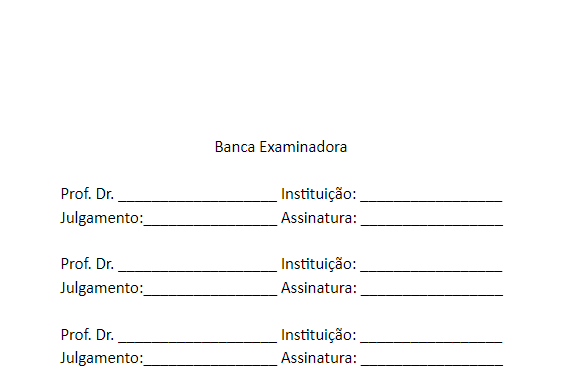
\includegraphics[scale=1]{folha_avaliacao2.png}
\end{figure}

\clearpage
% ---
% RESUMOS
% ---

% resumo em português
\setlength{\absparsep}{18pt} % ajusta o espaçamento dos parágrafos do resumo
\begin{resumo}

%-------------------------------------------------------------------------
A esfera pública, espaço de discussão democrática da sociedade, sofre mudanças constantes. A internet de certo ajudou a ampliar a participação das pessoas, mas seus filtros de conteúdo tem prejudicado o acesso à todas informações. O viés de confirmação, que intensifica a polarização política, juntamente com estes filtros intensificam um fenômeno chamado "Filtro bolha". Este trabalho busca encontrar uma forma de demonstrar ao usuário como ele está inserido neste contexto, demonstrando dados que ajudam a formar parte da informação que ele recebe de seu Facebook. Apesar do desenvolvimento de todas as funcionalidades necessárias, mudanças constantes na política de acesso à informação do Facebook impediram deixar este trabalho público, de forma com que seu acesso ainda deve ser controlado por adição de usuários teste, de forma manual. Porém, mesmo lançado publicamente, inferir conclusões sobre a base de dados acumulada, poderia ter uma precisão questionável, já que é dificil manter uma amostra sem qualquer viés.

Palavras-chaves: Filtro. Bolha. Viés. Confirmação. Facebook. Pública. 
\end{resumo}

% resumo em inglês
%-------------------------------------------------------------------------
% Informações sobre ``resumo em inglês''
% 
% Caso o projeto inteiro seja elaborada no idioma inglês, 
% então o ``Abstract'' vem antes do ``Resumo''.
% 
%-------------------------------------------------------------------------
\begin{resumo}[Abstract]
\begin{otherlanguage*}{english}
%-------------------------------------------------------------------------
The public sphere, democratic discussion place, is always changing. The internet helped to extend the people participation, but yours content filters has harmed the information access. The confirmation bias, that intensifies the political polarization, combined with this filters, intensifies a phenomenon called “Bubble Filter”. This work tries to find a way to show to the user how he is inserted on this context, showing data that is used to filter part of the information that he receives from Facebook. Despite the development of all necessary functionalities, constant changes on the Facebook’s access information policy prevented to put this work publicly, so that you access still need be controlled by adding manually the test user. Although, even if the work was already on public access, making conclusions of the data would be questionable, since that it’s hard to keep a sample without any bias. 

Keywords: Filter. Bubble. Bias. Confirmation. Facebook. Public.
\end{otherlanguage*}
\end{resumo}

% ---
% ---
% inserir lista de figuras
% ---
\pdfbookmark[0]{\listfigurename}{lof}
\listoffigures*
\cleardoublepage
% ---

% ---
% inserir lista de tabelas
% ---
\pdfbookmark[0]{\listtablename}{lot}
\listoftables*
\cleardoublepage
% ---

% ---
% inserir lista de abreviaturas e siglas
% ---
%-------------------------------------------------------------------------
% Informações sobre ``Lista de abreviaturas 
% e siglas'': 
%
% Opcional.
% Uma vez que se deseja usar, é necessário manter padrão e consistência no
% trabalho inteiro.
% Se usar: inserir em ordem alfabética.
%
%-------------------------------------------------------------------------
\begin{siglas}
  \item[WEB] Termo referente à \textit{World Wide Web}, geralmente referido como sinônimo de internet;
  \item[REST] Acrônimo para \textit{Representational State Transfer}. Arquitetura para servidores \textit{web};
  \item[API] Acrônimo para \textit{Application Programming Interface}. Interface de programação definida para o consumo da mesma;
  \item[TSE] Tribunal Superior Eleitoral. Órgão público responsável pelas eleições nacionais.
\end{siglas}
% ---

% ---

% ---
% inserir o sumario
% ---
\pdfbookmark[0]{\contentsname}{toc}
\tableofcontents*
\cleardoublepage
% ---

% ----------------------------------------------------------
% ELEMENTOS TEXTUAIS
% ----------------------------------------------------------
\textual



%-------------------------------------------------------------------------
% Informações sobre ``títulos de seções''
% 
% Para todos os títulos (seções, subseções, tabelas, ilustrações, etc):
%
% Em maiúscula apenas a primeira letra da sentença (do título), exceto 
% nomes próprios, geográficos, institucionais ou Programas ou Projetos ou
% siglas, os quais podem ter letras em maiúscula também.
%
%-------------------------------------------------------------------------
\chapter{Introdução}
\label{sec:intro}

Através dos anos, a sociologia estudou formas de tomadas de decisão em conjunto. Um conceito muito tratado foi o de 'Esfera Pública', definido por \citeonline{habermas} como um espaço democrático onde pessoas se reunem para tomar decisões que afetam o conjunto todo. Nesta esfera pública, onde o individuo de natureza privada externa suas preocupações, opiniões e posições, são criadas medidas para sanar os problemas propostos. Salienta-se também que o individuo só esta apto a participar de tal esfera caso seja um leitor das mídias institucionais. Refere-se inicialmente a burguesia como a classe instruída, e posteriormente dá como difusora de conhecimento a imprensa, que permite com que mais individuos estejam a par de problemas que aflijam tanto seu conjunto privado, portanto menor, quanto seu conjunto público, mais abrangente. Assim, através de uma gama de decisões tomadas pela moral do conjunto de individuos da esfera pública, a política institucional, representadas por instutuições governamentais, criam mecanismos (leis) para que a decisão tomada na esfera pública seja replicada para todos os individuos. Habermas também cita que muitas vezes, representantes de um conjunto de ideias e anseios podem ser alçados para retransmitir as ideias à esfera pública, seja pelo seu maior poder de comunicação, seja pelo seu maior conhecimento sobre o assunto. 

Este conceito já foi muito questionado na comunidade acadêmica, e sofreu correções do próprio Habermas, conforme aponta \citeonline{losekann}. Mas mesmo seus maiores críticos convergem ao fato de que apesar da análise geral de Habermas não cobrir as especificidades de cada sociedade, ainda sim coincidem com as formas com que a comunidade hoje toma suas decisões, apesar da participação dentro da esfera pública ter mudado drasticamente em tão pouco tempo.

Se antes \citeonline{habermas} considerava mídias institucionais e imprensa como difusores democráticas de informação, que fariam com que mais individuos fossem considerados leitores e pudessem participar das discussões da esfera pública, a internet rapidamente tratou de aumentar exponencialmente esta democratização. Segundo o Instituto Jornalístico Reuters \cite{reuters}, cerca de 66\% dos jovens no Brasil buscam como fonte de informação imediata (acontecimentos da ultima semana) pelas redes sociais. Mesmo em faixas etárias maiores, quando analisados no mercado mundial, mais de 1/3 das pessoas utilizam-se das redes sociais como forma de informação.

E as transformações políticas na esfera pública causadas pela internet não tardaram a ocorrer. A Primavera Árabe, conhecido fenômeno social que se iniciou em 2010, teve como principal ator a comunicação por redes sociais, como apontam alguns autores \cite{vivian,ferabolli}. As comunicações entre os agentes políticos da esfera pública daquela região ocorreu de forma livre, e a moral criada através das decisões tomadas em conjuto logo ocasionaram mudanças cenário político da região. 

O mesmo ocorreu na China \cite{liu}, onde diversas pesquisas demonstraram que mesmo em um país de partido único, a participação massiva de usuários nas redes sociais (mais de 700 milhões de usuários) causaram uma abertura maior do Partido Comunista. Corroboram também com a ideia de Habermas, que os participantes da esfera pública são os leitores ativos da mídia, tendo em vista que o aumento de participação na vida política era provenitente dos individuos que mais utilizavam internet.

Aumenta-se, porém, na mesma medida, a quantidade de dados disponíveis na internet. Um estudo feito pelo \citeonline{facebook_media} revela que exitiam em 2015 um total de 3.2 bilhões de usuários conectados, aproximadamente 5 bilhões de \textit{gigabytes} a cada dois dias \cite{parisier_data}. Com essa quantidade enorme de dados disponível, fica impossível a navegação na rede sem um filtro que traga ao usuário as informações que ele deseja. 

Por isso empresas como o Google, Facebook e outras tem mecanismos que visam filtrar as informações levadas até o usuário. Atavés de \textit{cookies} que armazenam as páginas visitadas pelo usuário, sites são capazes de trazer conteúdos personalizados a cada individuo. 

Esta personalização se dá tanto em mecanismos de pesquisa (Google, Yahoo, Microsoft Bing, etc), como em redes sociais. Estas por sua vez possuem um mecanismo diferente de filtro. Suas páginas trazem o conceito de \textit{feed} de notícias, que contém as informações mais relevantes ao usuário. Assim, as informações que possuem uma posição privilegiada são dados aprovados repetidamente pelo próprio usuário, que "curte" os \textit{posts}. Assim, a rede assume que o usuário possui mais interesses em \textit{posts} desta temática, e traz mais conteúdo relacionado para ele \cite{luckerson,parisier}.

Se aplicarmos este conceito à discussão política na esfera pública, podemos entender que o usuário na rede social receberá predominantemente informações que foram previamente aprovadas por ele. Imagina-se que um usuário, com posições morais e políticas definidas aprovará apenas informações que corroborem com a sua visão prévia. É o que define \citeonline{charles} em uma das primeiras pesquisas relacionadas ao chamado "Viés de Confirmação". O estudo realizado na Universidade de Stanford concluiu que pessoas possuem um viés muito forte em questões sociais relevantes, baseada em informações e experiências de vida prévias. Assim, novas informações contrárias ao ponto de vista pré-estabelecido tendem a serem instintivamente refutadas, sem qualquer análise crítica sobre as informações recebidas. 

Logo, com o filtro das redes sociais agindo com base nas informações recebidas de um usuário com tendências políticas enviesadas, pode causar um isolamento de informação ao usuário. A isso, \citeonline{parisier} chama de "Filtro Bolha", que une os conceitos de Viés de Confirmação e personalização da internet para o usuário, demonstrando que a navegação na rede de computadores pode ocorrer em uma bolha isolada de informações. Parisier ainda ressalta que a polarização política tende a se acentuar, apoiando-se na ideia de que o viés de confirmação apenas acentua o posicionamento ao extremo do individuo. 

\citeonline{mercier} cita que em algumas pesquisas, o individuo quando apresentado à ideia de que está emitindo opiniões sob o efeito do viés de confirmação, pode eventualmente contrariar e refutar essa ideia, demonstrando-se mais aberto a opiniões contrárias a outros temas. Anos antes, \citeonline{parisier} já dizia que alguma ação tecnológica deveria ser tomada por parte dos provedores de pesquisa e redes sociais para diminuir os efeitos do filtro bolha, ou ao menos mesclar bolhas de informação para amenizar seu extremismo. Pensando nisso, o Facebook anunciou em 2017 que faria alterações em sua plataforma para ajudar o usuário a ter acesso à contra-pontos \cite{facebook_related}, mas ainda há muito o que fazer.


\chapter{Objetivo}
\section{Objetivo Geral}

Construir uma ferramenta que auxilie o usuário a entender os efeitos do Filtro Bolha e do Viés de Confirmação no seu dia-a-dia, aplicado ao seu perfil na rede social Facebook, um possivel local de busca de informações. Será possível também a percepção do usuário sobre seu posicionamento político, juntamente com qual tipo de informação ele tem acesso por suas conexões na rede social. Como consequência, será possível ter uma base de dados com informações geográficas e demográficas de posicionamento político na esfera pública. 


\section{Objetivos Específicos}

\begin{itemize}
	\item{Possibilitar a percepção do usuário sobre os efeitos do chamado “Filtro Bolha”, entendendo suas aplicações;}
	\item{Iniciar a criação de uma base de dados que permita no futuro inferir algum tipo de informação baseado em dados geográficos e demográficos.}
\end{itemize}


\chapter{Revisão Bibliográfica}

Nesta seção será inserida uma descrição breve de cada item utilizado na Metodologia, e do material de estudo utilizado para a implementação da aplicação.

\section{REST}
REST é um acrônimo em inglês para as palavras "\textit{Representational State Transfer}". Trata-se de uma arquitetura muito utilizada em aplicações de servidor para um fácil e intuitivo acesso aos dados. Como forma de extensão da aplicação, foi utilizada uma arquitetura REST que será explicada na seção \ref{resultados} e documentada no apêndice \ref{apendiceA}.

\section{Node JS}
O servidor escolhido para a aplicação foi o Node JS, um projeto \textit{open source} que permite que scripts feitos em JavaScript rodem em aplicações servidor \textit{desktop}. Toda sua arquitetura é baseada em execução de tarefas assíncronas, juntamente com conceitos de troca de \textit{threads} em pontos de interrupção do Sistema Operacional, o que faz com que sua execução seja mais eficaz, sobretudo em aplicações \textit{web}.

\section{Sequelize}
O Sequelize é um \textit{framework} de ORM (\textit{Object-Relational Mapping}) do Node JS. Utiliza uma arquitetura baseada no conceito de \textit{Active Record}. Como a aplicação requer uma série de consultas com muitas junções de tabelas diferentes, as consultas do Sequelize são simples de implementar, agilizando o processo de desenvolvimento. Há também um controle de transação com o Banco de Dados implicito no \textit{framework}, o que dá uma maior robustez à aplicação. 

\section{Git/Github}
O sistema de versionamento escolhido para o projeto foi o git. Projeto iniciado em 2005, o git é um sistema de controle de versão open-source. A hospedagem desse repositório fica por conta do Github, site que é amplamente utilizado pela comunidade, sobretudo para projetos open-source. 

\section{Heroku}
A hospedagem da aplicação ficou por conta do Heroku, um servidor que permite com que aplicações de pequeno porte possam ser hospedadas de maneira gratuita. O site oferece estruturas de \textit{deploy} automáticos, já conectados com repositórios git ou svn. 

\section{Postgres}
O SGBD escolhido foi o Postgres, já que é o único SGBD gratuito disponível no Heroku. O Postgres é um projeto open-source, amplamente utilizado no mercado. 

\section{Graph API}
A API fornecida pelo Facebook para a consulta de dados de usuários e páginas é a Graph API. Para a utilização da Graph API, é necessário que o desenvolvedor crie um novo aplicativo, com uma chave secreta, dentro da sua conta de desenvolvedor do Facebook. Assim, sua aplicação \textit{web} está apta a utilizar a Graph API. A utilização básica é gratuíta.

\chapter{Metodologia}
\label{metodologia}

O projeto visa construir uma interface que permita ao usuário entender sua posição na bolha de informação em comparação com a polarização política de esquerda e direita. Foram inseridas 493 páginas de uma base de dados fornecida pelo Professor Dr. Márcio Moretto, que participa do projeto "Monitor do Debate Político no meio digital" \cite{monitor}. Essa base foi um resultado da pesquisa realizada pelo professor, que apontou as principais páginas do Facebook que tinham um alto nível de engajamento público. Esse engajamento era medido por número de compartilhamento da página e de seus posts por usuários, número de "curtir" na página e nos seus posts, número de comentários, etc. Através destas analises, também foi possível relacionar paginas às outras, consideram quais compartilhavam conteúdos entre si, quais haviam se "curtido", etc. Com as principais páginas definidas, houve um trabalho de qualificação dessas páginas, de forma que foram classificadas com \textit{tags} que definem o seu propósito na rede. 

Através destas \textit{tags} foi possível inferir o posicionamento político de cada uma das páginas. A tabela \ref{tab:tabelaTags} demonstra como foi feita a relação entre as tags existentes e o posicionamento político de cada uma.  

\begin{table}[htbp]
	\centering
	\caption{Relação entre as \textit{tags} existentes e o seu posicionamento político na esfera pública}
		\begin{tabular}{p{2in} p{2in} } \hline
			Posicionamento 	& Tags \\ \hline
			Esquerda		& Esquerda, anti-antiPT \\
			Direita			& Direita, anti-PT \\
			Imprensa		& Grande Imprensa, Jornais Digitais, Jornais Impressos, Televisão \\
			Neutro			& Outras tags/sem tags \\ \hline
		\end{tabular}
		\label{tab:tabelaTags}
\end{table}

A definição do posicionamento das páginas, apesar de não estar na estrutura inicial do dado, foi inserido no banco de dados para que se pudesse fazer a seleção dos dados já orientado a esse posicionamento. 

A aplicação desenvolvida consiste no uso da Graph API, que pede autorização ao usuário para ter acesso aos dados de localização, data de nascimento, amigos, páginas curtidas e gênero. Assim, é possivel cruzar os dados de páginas curtidas com a base prévia de páginas já posicionadas no espectro político da esfera pública, além de poder ter uma base geográfica demográfica desses posicionamentos.

Como as páginas são criadoras de conteúdo no Facebook, pode-se afirmar que todo o seu conteúdo produzido é de acordo com a sua posição política. Assim, o usuário terá acesso as postagens criadas por páginas que ele acompanha (pois ele curtiu estas páginas). Mas também terá acesso ao conteúdo das páginas em que seus amigos por sua vez estão seguindo. Logo, se um usuário segue muitas páginas classificadas como "Esquerda", espera-se que ele tenha um acesso mais fácil a conteúdos do espectro político da esquerda, ao passo que se ele possui muitos amigos que acompanham páginas de direita, ele tem o contraponto de que pode entrar em contato com postagens de conteúdo do espectro político de direita.

\chapter{Resultados}
\label{resultados}

A aplicação foi desenvolvida, tanto a visualização do usuário, quanto a API para a recuperação dos dados demográficos, conforme as imagens \ref{fig:figura1} e \ref{fig:figura2}. O código da aplicação é público e pode ser encontrado em https://github.com/brunomurozaki/bubbletest, onde há instruções rodar o servidor. A aplicação de visualização do usuário pode ser acessada em https://devbubbletest.herokuapp.com.

Entretando, vale ressaltar que a aplicação utiliza-se de permissões pedidas ao usuário na ação do login. Essas permissões precisam passar por autorização de utilização do Facebook, e para isso, é necessário a gravação de um vídeo onde deve-se demonstrar como os dados da determinada permissão são utilizados pela aplicação. Uma demonstração de como deve ser feita a requisição, com descrição completa dos passos que deve-se seguir para executar a aplicação, pode ser vista no apêndice \ref{apendiceA}. Após diversas tentativas, não foi possivel ainda conseguir as autorizações do Facebook para se usar as permissões de maneira pública. Portanto, para poder testar a aplicação inteira, é preciso ser adicionado como usuário teste da aplicação, e ser um contato válido do desenvolvedor que criou a requisição de teste (ser Amigo no Facebook). Caso esse processo seja completado, é possivel testar a aplicação. As imagens demonstram a aplicação com usuários teste adicionados por este processo citado.

\begin{figure}[H]
	\centering
	\caption{Layout da análise de posicionamento na esfera pública}
	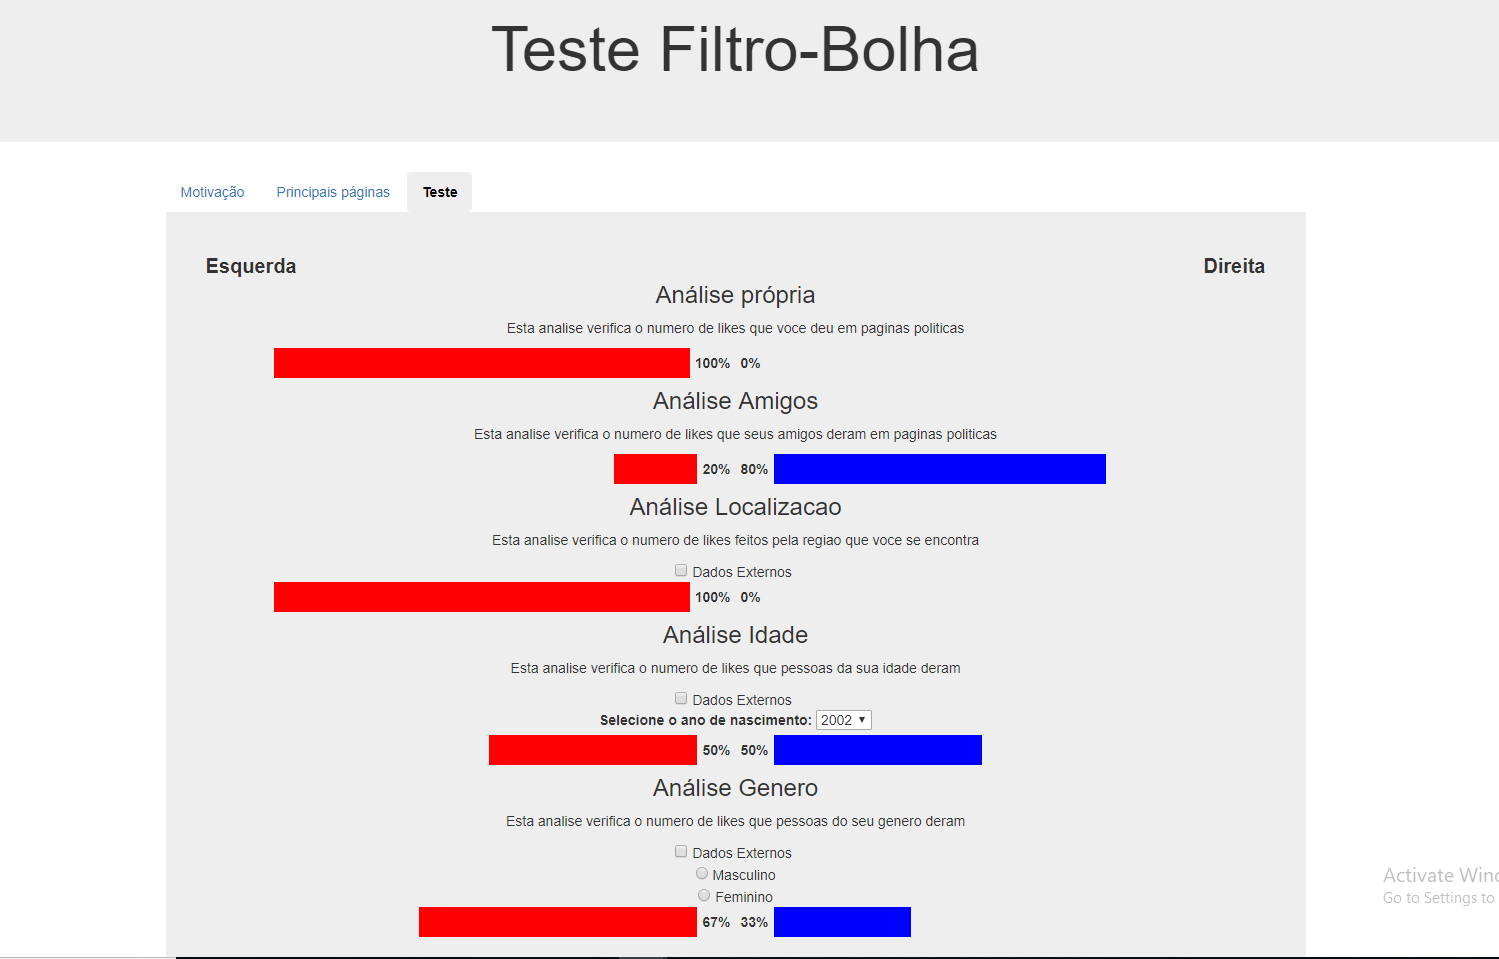
\includegraphics[scale=0.4]{figura1.png}
	\label{fig:figura1}
\end{figure}

\begin{figure}[H]
	\centering
	\caption{Exemplo de chamada REST para a listagem de dados no servidor}
	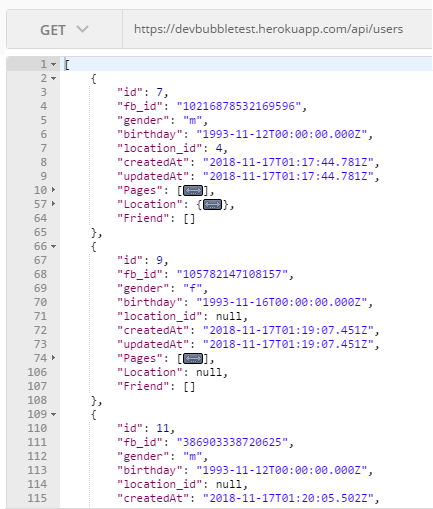
\includegraphics[scale=0.7]{figura2.png}
	\label{fig:figura2}
\end{figure}

Outro ponto a se salientar é o fato de que a avaliação de posicionamento politico das amizades do usuário se refere apenas aos que estão conectados no app. As amizades do usuário que não aprovaram as permissões da aplicação, não aparecem como conexão do usuário. Este é um bloqueio explícito do Facebook na Graph API. Entretando, a análise de dados relacionada à localização e gênero independem da conexão ou não com o usuário. Como todo usuário é adicionado a base de dados do projeto quando entra na aplicação, tem-se as informações demográficas e geográficas persistidas no banco. O modelo de banco utilizado é o descrito na imagem \ref{fig:bancoDeDados}.

\begin{figure}[H]
	\centering
	\caption{Definição do banco de dados utilizado pela aplicação}
	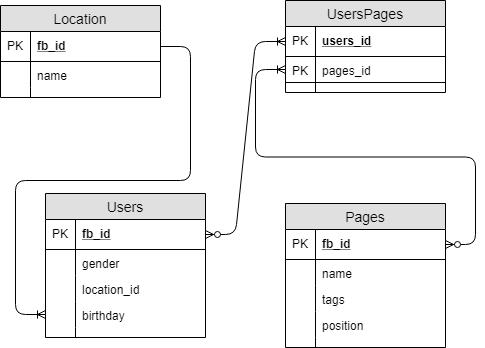
\includegraphics[scale=0.7]{banco_de_dados.png}
	\label{fig:bancoDeDados}
\end{figure}


Além da visualização relacionadas ao perfil do usuário, há também a possibilidade de se comparar os dados apresentados pela aplicação com dados externos, de fora da aplicação do Facebook. Cada estado possui os dados da última eleição (segundo turno), fornecidos pelo \citeonline{tse} e os dados sobre a última pesquisa de opinião realizada pelo \citeonline{datafolha}, já que o TSE não disponibiliza dados sobre o gênero, localidade e idade de quem votou. 

Quanto aos dados demográficos e geográficos armazenados, todos podem ser acessados pela API localizada no mesmo endereço da aplicação. No Apêndice \ref{apendiceA} é possivel ver todos as chamadas possiveis dentro da API, juntamente com os resultados esperados. 

\chapter{Discussão}

Tirando-se as dificuldades de desenvolvimento, que impediram a aplicação de ser lançada publicamente, não apenas para usuários pré-aprovados, inferir conclusões através dos dados seria extremamente difícil. Inicialmente, o plano do projeto era uma ampla divulgação em páginas de temáticas políticas, para que se tivesse uma amostra bem grande, e uma divulgação ampla em páginas dos dois lados do espectro político da esfera pública. Porém, mesmo desta forma, fica difícil garantir uma amostra sem viés. 

Quanto a análise do usuário, a análise por amizades e páginas curtidas é eficaz pois considera quem cria conteúdos e quem potencialmente os compartilha. Porém, o universo de amigos se restringe apenas aos presentes na aplicação, e também se desconsidera totalmente o algorítimo que fornece o conteúdo ao usuário, feito pelo Facebook. Alguns testes realizados mostram que após um tempo elevado de conexão no Facebook, muitas vezes é trazido um conteúdo pouco comum ao usuário, já que o tempo elevado na aplicação o fez percorrer por todas as temáticas que já lhe são familiares. Existem outros fatores, como engajamento em postagens de amigos por meio de comentários, que fazem também com que o Facebook considere que aquele conteúdo é algo que te interessa e que vale a pena lhe trazer novamente. Há também o fator de \textit{marketing} pago, que a aplicação do projeto não cobre. Uma melhor análise poderia ser feita se fosse possível uma análise do conteúdo trazido pelo Facebook diretamente. Tal funcionalidade existe na Graph API, porém nos últimos anos foi restringida a fabricantes de aplicativos nativos do Facebook, como empresas de telefonia. No anexo \ref{anexoA}, fugura \ref{fig:request}, é possível ver uma das diversas tentativas de contato com a equipe de desenvolvimento do projeto, explicando o porquê seria interessante a liberação desta permissão para a aplicação. Não foi obtido sucesso na requisição.

Outro ponto que foi tratado durante o desenvolvimento do projeto foi a implementação da autenticação por \textit{token}, ou \textit{OAuth}. Este tipo de autenticação com o servidor foi por um tempo pré-requisito do Facebook, mas posteriormente esse requisito foi retirado. A preocupação do Facebook era que o \textit{id} do usuário fornecido pela Graph API, apesar de diferente entre as aplicações, era possivel acessar o perfil da pessoa diretamente, colocando este \textit{id} na \textit{url}. Porém, uma atualização recente da Graph API fez com que o \textit{id} não seja mais o localizador do perfil quando inserido diretamente na \textit{url}.

Por último, vale também salientar as constantes mudanças que o Facebook tem feito em sua política de acesso à informação. Muitas das permissões antes disponíveis se tornaram obsoletas, e outras tiveram a dificuldade de acesso aumentada. Tudo isso se refere aos recentes problemas que a empresa teve nas questões de privacidade dos usuários, como o vazamento de informação de perfis, Cambridge Analítica, e outros \cite{cambridge1,cambridge2,breach}

\chapter{Conclusão}

Os dados cada vez mais apontam uma migração de busca por informação da mídia tradicional (rádio, televisão, jornal) para a Internet. Mais do que isso. As redes sociais tem tido o papel de informar os usuários da Internet. Apesar de ser nocivo ao acesso à informação, os filtros inseridos pelas redes sociais são necessários para a manutenção do usuário na rede. Porém, é necessária a ação por parte dessas empresas e da comunidade em geral para amenizar os efeitos deste Filtro Bolha.

Este trabalho tentou demonstrar uma dessas formas, informando ao usuário sobre os problemas trazidos pelo filtro de conteúdo, e como ele é formado com a ajuda do viés de confirmação. Porém, mesmo com todas as dificuldades apresentadas, o esforço ainda seria insuficiente. Deve-se levar em consideração ainda pontos específicos de cada plataforma. Questionamentos sobre como o Algoritimo do Facebook funciona, ou até de outras redes sociais, são pontos que ajudariam a comunidade a entender como estes filtros funcionam, e quais as possiveis abordagens são necessárias para amenizar estes efeitos. 

Nota-se também um esforço grande por parte do Facebook de rever sua política de privacidade, que de certa forma infere diretamente em como o usuário lida com a rede. Demonstra também que a empresa sabe o tamanho que atingiu, e o poder de influência dentro da esfera púlica que ela tem. Após os escândalos envolvendo a empresa, seus diretores tem tentado abrir mais sua plataforma, demonstrando seus métodos de segurança, e aprimorando o acesso às informações. Caminha-se assim talvez para um entendimento comum de como a rede deve restringir sua participação na sociedade para que não haja nocividade à democracia.  

% ----------------------------------------------------------
% ELEMENTOS PÓS-TEXTUAIS
% ----------------------------------------------------------
\postextual
% ----------------------------------------------------------

% ----------------------------------------------------------
% Referências bibliográficas
% ----------------------------------------------------------
\bibliography{referencias}

% ----------------------------------------------------------
% Glossário
% ----------------------------------------------------------
%
% Consulte o manual da classe abntex2 para orientações sobre o glossário.
%
%\glossary

% ----------------------------------------------------------
% Apêndices
% ----------------------------------------------------------

% ---
% Inicia os apêndices
% ---
\begin{apendicesenv}

% Imprime uma página indicando o início dos apêndices
%\partapendices

%-------------------------------------------------------------------------
% Informações sobre ``apêndice''
%
% Para todos os captions/(títulos) (de seções, subseções, tabelas, 
% ilustrações, etc):
%     - em maiúscula apenas a primeira letra da sentença (do título), 
%       exceto nomes próprios, geográficos, institucionais ou Programas ou
%       Projetos ou siglas, os quais podem ter letras em maiúscula também.
%
% Todas  as tabelas, ilustrações (figuras, quadros, gráficos, etc. ), 
% anexos, apêndices devem obrigatoriamente ser citados no texto.
%      - a citação deve vir sempre antes da primeira vez em que a tabela, 
%        ilustração, etc., aparecer pela primeira vez.
%
%-------------------------------------------------------------------------
\chapter{Chamadas REST para a API}
\label{apendiceA}

Neste apêndice será apresentada a lista de chamadas REST para a API de acesso aos dados geográficos e demográficos, bem como o resultado gerado por estas chamadas. Como já tratado anteriormente, o servidor não possui qualquer tipo de autenticação, já que o Facebook mudou sua política recentemente, fazendo que o identificador único de perfil fosse relevante somente para a aplicação, não mais para o acesso direto ao site. Cada chamada será explicada em uma seção separada, identificada inicialmente pelo seu título, seguido pelo método \textit{HTTP} utilizado, a \textit{url} de chamada e os parâmetros, caso necessário.

\textbf{Nota: } As \textit{urls} que possuem campos como ":campo" em seus endereços indicam que devem receber um parâmetro variável em seu conteúdo, diretamente enviado pela \textit{url}.

\section*{1.1 Listagem de Usuários}

\begin{itemize}
	\item {GET} \textit{/api/users}
\end{itemize}

Chamada REST utilizada para a listagem de todos os usuários cadastrados no banco de dados. O resultado também inclui a localização do usuário e também todas as páginas curtidas. O exemplo de retorno pode ser visualizado na imagem \ref{fig:retornoUsers}.

\begin{figure}[H]
	\centering
	\caption{Resultado parcial da chamada de listagem de usuários}
	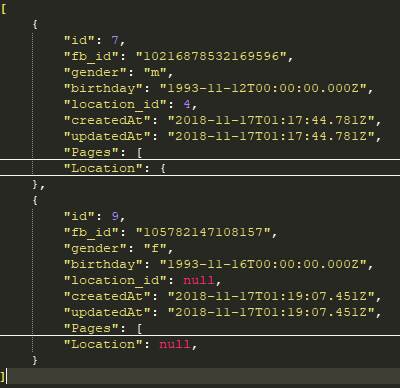
\includegraphics[scale=1]{resultadoUsers.png}
	\label{fig:retornoUsers}
\end{figure}


\section*{1.2 Inserção de Usuários}

\begin{itemize}
	\item {POST} \textit{/api/users}
\end{itemize}

Chamada REST para a inserção do usuário no banco de dados. Os parâmetros passados no corpo da requisição \textit{HTTP} devem ser como descritos na tabela \ref{tab:tabelaBodyUsers}. Não há retorno para esta chamada.

 \begin{table}[htbp]
 	\centering
 	\caption{Parâmetos para a chamada REST de inserção de Usuário}
 	\begin{tabular}{p{1.5in} p{1in} p{1in} p{1.5in}  } \hline
 		Nome do Campo 		& 		Obrigatório 		& 		Tipo 		&		 Descrição \\ \hline
 		fb\_id				& 		Sim					&	Caracter		& Identificador único do perfil do Facebook do usuário (tem valor apenas dentro da aplicação) \\
 		gender				& 		Não					& Caracter (1)		& Caracter unico de identificação do gênero do usuário \\
 		birthday			& 		Não					& Data				& Data de nascimento do usuário \\
 		location\_id		& 		Não					& Caracter			& Identificador dado pelo Facebook de localização do usuário
 	\end{tabular}
  	\label{tab:tabelaBodyUsers}
 \end{table}

\section*{1.3 Numero de "curtir" em páginas políticas por gênero}

\begin{itemize}
	\item {GET} \textit{/api/users/:gender}
\end{itemize}

Chamada REST para recuperar o número de "curtir" em páginas poíticas, por gênero. A tabela \ref{tab:tabelaGender} demonstra o parâmetro para a utilização desta chamada. A imagem \ref{fig:retornoGender} demonstra o retorno da chamada.

 \begin{table}[htbp]
	\centering
	\caption{Parâmeto para a chamada de pesquisa de páginas políticas por gênero}
	\begin{tabular}{p{1.5in} p{1in} p{1in} p{1.5in}  } \hline
		Nome do Campo 		& 		Obrigatório 		& 		Tipo 		&		 Descrição \\ \hline
		gender				& 		Sim					& Caracter (1)		&
		Caracter unico para a definiçao do gênero a ser procurado ('m' ou 'f') 
	\end{tabular}
	\label{tab:tabelaGender}
\end{table}

\begin{figure}[H]
	\centering
	\caption{Resultado da chamada de "curtir" por gêneros (exemplo de chamada com o parâmetro 'm')}
	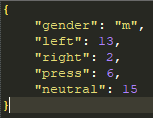
\includegraphics[scale=1]{resultadoGender.png}
	\label{fig:retornoGender}
\end{figure}


\section*{1.4 Páginas curtidas por usuário}

\begin{itemize}
	\item {GET} \textit{/api/users/:id/likes}
\end{itemize}

Chamada REST para retorno da lista de páginas políticas curtidas pelo usuário pelo id enviado como parâmetro. A tabela \ref{tab:tabelaUserLike} descreve o parâmetro a ser enviado. A imagem \ref{fig:retornoUserLike} exemplifica o retorno desta chamada.

 \begin{table}[htbp]
	\centering
	\caption{Parâmeto para a chamada de recuperação de páginas curtidas por usuário}
	\begin{tabular}{p{1.5in} p{1in} p{1in} p{1.5in}  } \hline
		Nome do Campo 		& 		Obrigatório 		& 		Tipo 		&		 Descrição \\ \hline
		id				& 		Sim					& Caracter 		&
		Cadeia de caracteres que representam o Facebook \textit{id} do usuário. Este \textit{id} é único e só é reconhecido por chamadas feitas pela aplicação do Facebook, não sendo útil quando chamado diretamente, pela \textit{url} do site.
	\end{tabular}
	\label{tab:tabelaUserLike}
\end{table}

\begin{figure}[H]
	\centering
	\caption{Resultado da chamada de "curtir" por usuário}
	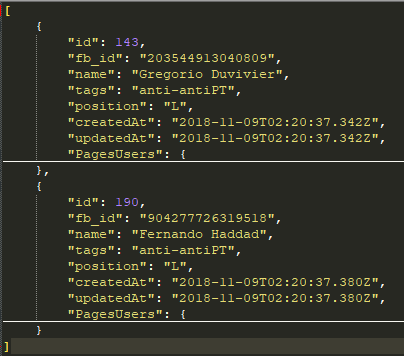
\includegraphics[scale=1]{resultadoUserLike.png}
	\label{fig:retornoUserLike}
\end{figure}

\section*{1.5 Numero de "curtir" em páginas políticas por usuário}

\begin{itemize}
	\item {GET} \textit{/api/users/:id/likesSummary}
\end{itemize}

Chamada REST para retorno do número de páginas curtidas por usuário, separadas pela sua posição política.  A tabela \ref{tab:tabelaUserLikeSummary} descreve o parâmetro a ser enviado. A imagem \ref{fig:retornoUserLikeSummary} exemplifica o retorno desta chamada.

 \begin{table}[htbp]
	\centering
	\caption{Parâmeto para a chamada de recuperação de resumo de páginas curtidas por usuário}
	\begin{tabular}{p{1.5in} p{1in} p{1in} p{1.5in}  } \hline
		Nome do Campo 		& 		Obrigatório 		& 		Tipo 		&		 Descrição \\ \hline
		id				& 		Sim					& Caracter 		&
		Cadeia de caracteres que representam o Facebook \textit{id} do usuário. Este \textit{id} é único e só é reconhecido por chamadas feitas pela aplicação do Facebook, não sendo útil quando chamado diretamente, pela \textit{url} do site.
	\end{tabular}
	\label{tab:tabelaUserLikeSummary}
\end{table}

\begin{figure}[H]
	\centering
	\caption{Resultado da chamada de resumo de páginas curtidas por usuário}
	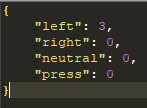
\includegraphics[scale=1]{resultadoUserLikeSummary.png}
	\label{fig:retornoUserLikeSummary}
\end{figure}

\section*{1.6 Numero de "curtir" em páginas políticas por idade}

\begin{itemize}
	\item {GET} \textit{/api/users/age/:birthday/likes}
\end{itemize}

Chamada REST para retorno do número de páginas políticas curtidas, separadas pelo seu posicionamento político. A tabela \ref{tab:tabelaBirthdayLikeSummary} descreve o parâmetro a ser enviado. A imagem \ref{fig:retornoBirthdayLikeSummary} exemplifica o retorno desta chamada.

 \begin{table}[htbp]
	\centering
	\caption{Parâmeto para a chamada de recuperação de resumo de páginas curtidas por data de nascimento}
	\begin{tabular}{p{1.5in} p{1in} p{1in} p{1.5in}  } \hline
		Nome do Campo 		& 		Obrigatório 		& 		Tipo 		&		 Descrição \\ \hline
		birthday				& 		Sim					& Data 		&
		Data de nascimento a ser pesquisada. \textbf{Nota: } No momento, a API trata apenas o ano de nascimento na pesquisa.
	\end{tabular}
	\label{tab:tabelaBirthdayLikeSummary}
\end{table}

\begin{figure}[H]
	\centering
	\caption{Resultado da chamada de resumo de número de curtidas por data de nascimento}
	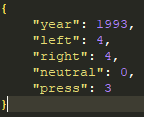
\includegraphics[scale=1]{resultadoBirthdayLikeSummary.png}
	\label{fig:retornoBirthdayLikeSummary}
\end{figure}

\section*{1.7 Listagem de localizações}

\begin{itemize}
	\item {GET} \textit{/api/location}
\end{itemize}

Chamada REST para a listagem de todas as localizações registradas. A imagem \ref{fig:retornoLocation} demonstra o resultado parcial desta chamada.

\begin{figure}[H]
	\centering
	\caption{Resultado da chamada de listagem de Localizações}
	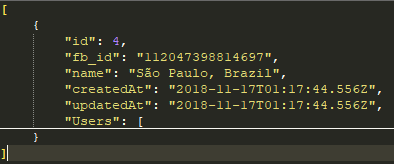
\includegraphics[scale=1]{resultadoLocation.png}
	\label{fig:retornoLocation}
\end{figure}


\section*{1.8 Inserção de localizações}

\begin{itemize}
	\item {POST} \textit{/api/location}
\end{itemize}

Chamada REST para a inserção de localização no banco de dados. A tabela \ref{tab:tabelaBodyLocation} descreve os parâmetros que devem ser enviados. Não há retorno para esta chamada.

 \begin{table}[htbp]
	\centering
	\caption{Parâmetos para a chamada REST de inserção de Usuário}
	\begin{tabular}{p{1.5in} p{1in} p{1in} p{1.5in}  } \hline
		Nome do Campo 		& 		Obrigatório 		& 		Tipo 		&		 Descrição \\ \hline
		fb\_id				& 		Sim					&	Caracter		& Identificador único da localização, dado pelo Facebook \\
		name				& 		Não					& 	Caracter 		& Nome da localização registrada no Facebook \\
	\end{tabular}
	\label{tab:tabelaBodyLocation}
\end{table}

\section*{1.9 Número de "curtir" em páginas políticas por localização}

\begin{itemize}
	\item {GET} \textit{/api/location/:id/likes}
\end{itemize}

Chamada REST para retorno do resumo de curtidas em páginas políticas, separadas pelo posicionamento político. A tabela \ref{tab:tabelaLocationLikeSummary} descreve o parâmetro a ser enviado. A imagem \ref{fig:retornoLocationLikeSummary} exemplifica o retorno desta chamada.

 \begin{table}[htbp]
	\centering
	\caption{Parâmeto para a chamada de recuperação de resumo de páginas curtidas por localização}
	\begin{tabular}{p{1.5in} p{1in} p{1in} p{1.5in}  } \hline
		Nome do Campo 		& 		Obrigatório 		& 		Tipo 		&		 Descrição \\ \hline
		id				& 		Sim					& Caracter 		&
		\textit{id} fornecido pelo Facebook da localização desejada. 
	\end{tabular}
	\label{tab:tabelaLocationLikeSummary}
\end{table}

\begin{figure}[H]
	\centering
	\caption{Resultado da chamada de resumo de número de curtidas por localização}
	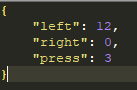
\includegraphics[scale=1]{resultadoLocationLikeSummary.png}
	\label{fig:retornoLocationLikeSummary}
\end{figure}

\section*{1.10 Listagem de Páginas}

\begin{itemize}
	\item {GET} \textit{/api/pages}
\end{itemize}

Chamada REST para a listagem de todas as páginas analisadas. A imagem \ref{fig:retornoPages} exemplifica o retorno desta chamada.

\begin{figure}[H]
	\centering
	\caption{Resultado da chamada de listagem de páginas}
	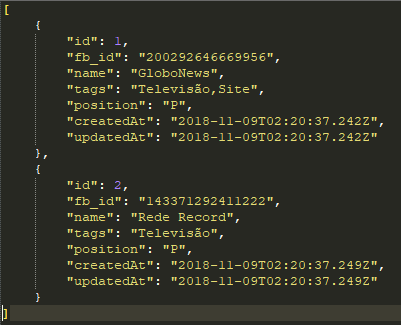
\includegraphics[scale=1]{resultadoPages.png}
	\label{fig:retornoPages}
\end{figure}

\section*{1.11 Inserção de "curtir" em páginas políticas}

\begin{itemize}
	\item {POST} \textit{/api/likes}
\end{itemize}

Chamada REST para inserção de "curtir" de um usuário em uma página. A tabela \ref{tab:tabelaLikeAdd} descreve os parâmetros a serem enviados. Não há retorno para esta chamada.

 \begin{table}[htbp]
	\centering
	\caption{Parâmetros para a inserção de "curtir" por um usuário}
	\begin{tabular}{p{1.5in} p{1in} p{1in} p{1.5in}  } \hline
		Nome do Campo 		& 		Obrigatório 		& 		Tipo 		&		 Descrição \\ \hline
		user\_id			& 		Sim					& Caracter 			&
		Cadeia de caracteres que representam o Facebook \textit{id} do usuário. Este \textit{id} é único e só é reconhecido por chamadas feitas pela aplicação do Facebook, não sendo útil quando chamado diretamente, pela \textit{url} do site. \\
		page\_id			&		Sim					& Caracter 			&        Cadeia de caracteres que identifica a página no Facebook. 		 
	\end{tabular}
	\label{tab:tabelaLikeAdd}
\end{table}


\end{apendicesenv}
% ---


% ----------------------------------------------------------
% Anexos
% ----------------------------------------------------------

% ---
% Inicia os anexos
% ---
\begin{anexosenv}

\chapter{Tratativas com a plataforma Facebook}
\label{anexoA}

Este anexo refere-se aos contatos realizados com a empresa para pedir autorização para utilizar-se de permissões fora do escopo, bem como as tentativas de tornar a aplicação pública. A requisição de autorização foi feita diversas vezes, e desde a última mudança na política da plataforma, nunca foram aprovadas.

\begin{figure}[H]
	\centering
	\caption{Requisição não aprovada pelo Facebook}
	
\includegraphics[scale=1]{not_approved1.png}
\end{figure}

\begin{figure}[H]
	\centering
	\caption{Informação de retirada de permissões previamente aprovadas pela nova política de acesso de informação do site}
	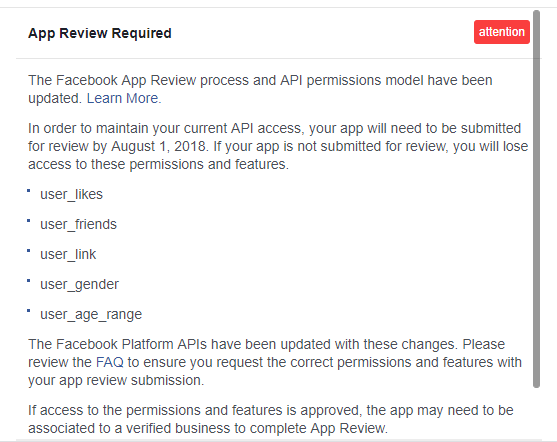
\includegraphics[scale=1]{app_verification.png}
\end{figure}

\begin{figure}[H]
	\centering
	\caption{Requisição feita para ter autorização de utulizar a permissão de \textit{feed} do Facebook}
	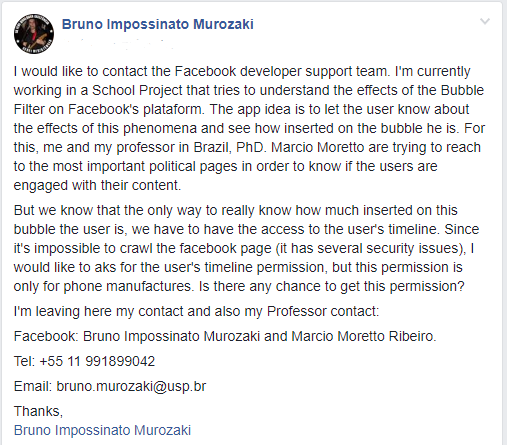
\includegraphics[scale=1]{request.png}
	\label{fig:request}
\end{figure}




\end{anexosenv}

%---------------------------------------------------------------------
% INDICE REMISSIVO
%---------------------------------------------------------------------
%%%%%MF\phantompart
%%%%%MF\printindex
%---------------------------------------------------------------------

\end{document}
